\documentclass{standalone}

%----------------------------------------------------------------------------------------------%
%                                 Packages and basic declarations
%----------------------------------------------------------------------------------------------%

\usepackage{tikz}
\usepackage{verbatim}
\usepackage{pgf}
\usepackage{tikz}
\usepackage{mathrsfs}

\usetikzlibrary{arrows}



%----------------------------------------------------------------------------------------------%
%----------------------------------------------------------------------------------------------%
%                                            DOCUMENT STARTS
%----------------------------------------------------------------------------------------------%
%----------------------------------------------------------------------------------------------%

\begin{document}

%----------------------------------------------------------------------------------------------%
%                Single RVE with applied constant strain, only debonded
%----------------------------------------------------------------------------------------------%
 
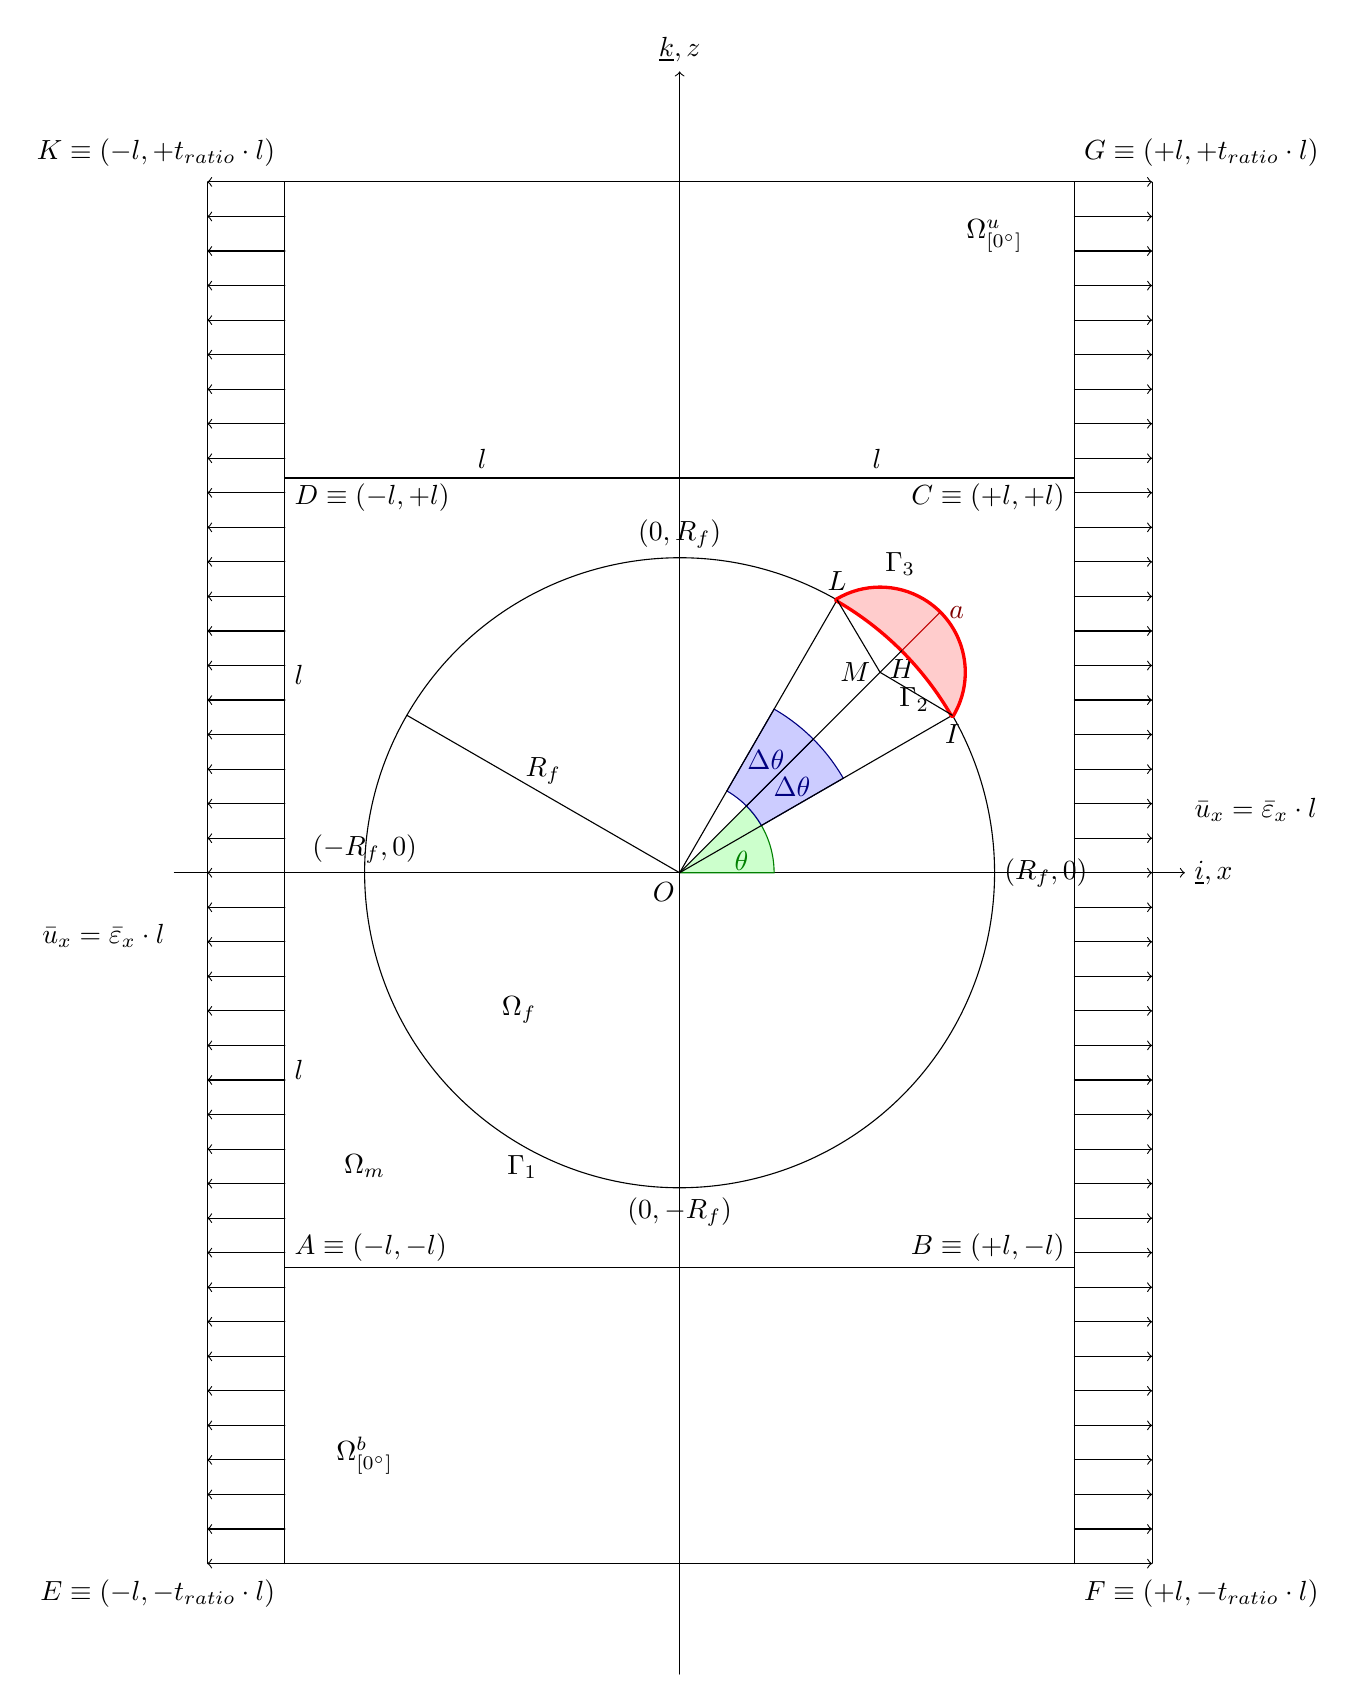
\begin{tikzpicture}[scale=4,cap=round,x=1cm,y=1cm]

%----------------------------------------------------------------------------------------------%
%                                          INPUT PARAMETERS
%----------------------------------------------------------------------------------------------%

\def\Rf{1}
\def\Vff{0.5}
\def\tratio{0.75}
\def\meshfacone{0.2}
\def\meshfactwo{0.75}
\def\meshfacthree{0.5}
\def\thetavalue{45}
\def\deltatheta{15}

%----------------------------------------------------------------------------------------------%
%                               Definition of dependent parameters
%----------------------------------------------------------------------------------------------%

\def\pivalue{3.141592653589793238462643383279502884197169399375105820974944592307816406286}

\newcommand{\half}[1]{
       0.5*#1
       }

\pgfmathsetmacro\l{0.5*\Rf*sqrt(\pivalue/\Vff)}

\def\domlim{1.28*\l}
\def\loadlim{1.197*\l}
\def\loadlabel{0.2*\Rf}
\def\cornerlabel{1.077*\l}

\def\thetabot{\thetavalue-\deltatheta}
\def\thetaup{\thetavalue+\deltatheta}

\def\thetahalfbot{\thetavalue-0.5*\deltatheta}
\def\thetahalfup{\thetavalue+0.5*\deltatheta}

\def\thetaround{360+\thetavalue-\deltatheta}
\def\thetadraw{0.25*\thetavalue}

\def\xM{0.9*\costheta*\Rf}
\def\yM{0.9*\sintheta*\Rf}

\pgfmathsetmacro\cosfourtyfive{cos(45)}
\pgfmathsetmacro\sinfourtyfive{sin(45)}

\pgfmathsetmacro\costheta{cos(\thetavalue)}
\pgfmathsetmacro\sintheta{sin(\thetavalue)}

\pgfmathsetmacro\costhetabot{cos(\thetabot)}
\pgfmathsetmacro\sinthetabot{sin(\thetabot)}

\pgfmathsetmacro\costhetaup{cos(\thetaup)}
\pgfmathsetmacro\sinthetaup{sin(\thetaup)}

\pgfmathsetmacro\costhetahalfbot{cos(\thetahalfbot)}
\pgfmathsetmacro\sinthetahalfbot{sin(\thetahalfbot)}

\pgfmathsetmacro\costhetahalfup{cos(\thetahalfup)}
\pgfmathsetmacro\sinthetahalfup{sin(\thetahalfup)}
  
\pgfmathsetmacro\yloadarrowone{\l+(\loadlim-\l)*0.2}
\pgfmathsetmacro\yloadarrowtwo{\l+2*(\loadlim-\l)*0.2}
\pgfmathsetmacro\yloadarrowthree{\l+3*(\loadlim-\l)*0.2}
\pgfmathsetmacro\yloadarrowfour{\l+4*(\loadlim-\l)*0.2}

\pgfmathsetmacro\ILsquared{(\costhetabot-\costhetaup)*(\costhetabot-\costhetaup)+(\sinthetabot-\sinthetaup)*(\sinthetabot-\sinthetaup))}
\pgfmathsetmacro\IMsquared{(\costhetabot-0.9*\costheta)*(\costhetabot-0.9*\costheta)+(\sinthetabot-0.9*\sintheta)*(\sinthetabot-0.9*\sintheta)}
\pgfmathsetmacro\IL{sqrt(\ILsquared)}
\pgfmathsetmacro\IM{sqrt(\IMsquared)}
\pgfmathsetmacro\angleM{asin(0.5*\IL/\IM)}

\def\crackstartangle{\thetavalue-\angleM}
\def\crackstopangle{\thetavalue+\angleM}

\pgfmathsetmacro\meshradiusone{\meshfactwo*\Rf}
\pgfmathsetmacro\meshradiustwo{\Rf+\meshfacthree*(\l-\Rf)}

\tikzstyle{axes}=[]

\draw (\costhetaup,\sinthetaup)arc (\thetaup:\thetaround:\Rf);

\begin{scope}[style=axes]
  \draw[->] (-\domlim,0) -- (\domlim,0) node[right] {$\underline{i}, x$};
  \draw[->] (0,-\domlim-\tratio*\l) -- (0,\domlim+\tratio*\l) node[above] {$\underline{k}, z$};
\end{scope}

\pgfmathsetmacro\ltot{\l+\tratio*\l}

 \draw[->] (\l, -\ltot) -- (\loadlim,-\ltot);
  \draw[->] (\l, -0.9*\ltot) -- (\loadlim, -0.9*\ltot);
 \draw[->] (\l, -0.8*\ltot) -- (\loadlim,-0.8*\ltot);
 \draw[->] (\l,-0.7*\ltot) -- (\loadlim,-0.7*\ltot);
 \draw[->] (\l,-0.6*\ltot) -- (\loadlim,-0.6*\ltot);
 \draw[->] (\l,-\half{\ltot}) -- (\loadlim,-\half{\ltot});
 \draw[->] (\l, -0.4*\ltot) -- (\loadlim, -0.4*\ltot);
 \draw[->] (\l,-0.3*\ltot) -- (\loadlim,-0.3*\ltot);
 \draw[->] (\l,-0.2*\ltot) -- (\loadlim,-0.2*\ltot);
 \draw[->] (\l,-0.1*\ltot) -- (\loadlim,-0.1*\ltot);
 \draw[->] (\l,-0.0*\ltot) -- (\loadlim,-0.0*\ltot);
 \draw[->] (\l,0.1*\ltot) -- (\loadlim,0.1*\ltot);
 \draw[->] (\l,0.2*\ltot) -- (\loadlim,0.2*\ltot);
 \draw[->] (\l,0.3*\ltot) -- (\loadlim,0.3*\ltot);
 \draw[->] (\l,0.4*\ltot) -- (\loadlim,0.4*\ltot);
 \draw[->] (\l,\half{\ltot}) -- (\loadlim,\half{\ltot});
 \draw[->] (\l,0.6*\ltot) -- (\loadlim,0.6*\ltot);
 \draw[->] (\l,0.7*\ltot) -- (\loadlim,0.7*\ltot);
 \draw[->] (\l,0.8*\ltot) -- (\loadlim,0.8*\ltot);
 \draw[->] (\l,0.9*\ltot) -- (\loadlim,0.9*\ltot);
 \draw[->] (\l, -0.95*\ltot) -- (\loadlim, -0.95*\ltot);
 \draw[->] (\l, -0.85*\ltot) -- (\loadlim,-0.85*\ltot);
 \draw[->] (\l,-0.75*\ltot) -- (\loadlim,-0.75*\ltot);
 \draw[->] (\l,-0.65*\ltot) -- (\loadlim,-0.65*\ltot);
 \draw[->] (\l,-0.55*\ltot) -- (\loadlim,-0.55*\ltot);
 \draw[->] (\l, -0.45*\ltot) -- (\loadlim, -0.45*\ltot);
 \draw[->] (\l,-0.35*\ltot) -- (\loadlim,-0.35*\ltot);
 \draw[->] (\l,-0.25*\ltot) -- (\loadlim,-0.25*\ltot);
 \draw[->] (\l,-0.15*\ltot) -- (\loadlim,-0.15*\ltot);
 \draw[->] (\l,-0.05*\ltot) -- (\loadlim,-0.05*\ltot);
 \draw[->] (\l,0.05*\ltot) -- (\loadlim,0.05*\ltot);
 \draw[->] (\l,0.15*\ltot) -- (\loadlim,0.15*\ltot);
 \draw[->] (\l,0.25*\ltot) -- (\loadlim,0.25*\ltot);
 \draw[->] (\l,0.35*\ltot) -- (\loadlim,0.35*\ltot);
 \draw[->] (\l,0.45*\ltot) -- (\loadlim,0.45*\ltot);
 \draw[->] (\l,0.55*\ltot) -- (\loadlim,0.55*\ltot);
 \draw[->] (\l,0.65*\ltot) -- (\loadlim,0.65*\ltot);
 \draw[->] (\l,0.75*\ltot) -- (\loadlim,0.75*\ltot);
 \draw[->] (\l,0.85*\ltot) -- (\loadlim,0.85*\ltot);
 \draw[->] (\l,0.95*\ltot) -- (\loadlim,0.95*\ltot);
 \draw[->] (\l,\ltot) -- (\loadlim,\ltot);
 
 \draw[->] (-\l,-\ltot) -- (-\loadlim,-\ltot);
  \draw[->] (-\l, -0.9*\ltot) -- (-\loadlim, -0.9*\ltot);
 \draw[->] (-\l,-0.8*\ltot) -- (-\loadlim,-0.8*\ltot);
 \draw[->] (-\l,-0.7*\ltot) -- (-\loadlim,-0.7*\ltot);
 \draw[->] (-\l,-0.6*\ltot) -- (-\loadlim,-0.6*\ltot);
 \draw[->] (-\l,-\half{\ltot}) -- (-\loadlim,-\half{\ltot});
 \draw[->] (-\l, -0.4*\ltot) -- (-\loadlim, -0.4*\ltot);
 \draw[->] (-\l,-0.3*\ltot) -- (-\loadlim,-0.3*\ltot);
 \draw[->] (-\l,-0.2*\ltot) -- (-\loadlim,-0.2*\ltot);
 \draw[->] (-\l,-0.1*\ltot) -- (-\loadlim,-0.1*\ltot);
 \draw[->] (-\l,-0.0*\ltot) -- (-\loadlim,-0.0*\ltot);
 \draw[->] (-\l,0.1*\ltot) -- (-\loadlim,0.1*\ltot);
 \draw[->] (-\l,0.2*\ltot) -- (-\loadlim,0.2*\ltot);
 \draw[->] (-\l,0.3*\ltot) -- (-\loadlim,0.3*\ltot);
 \draw[->] (-\l,0.4*\ltot) -- (-\loadlim,0.4*\ltot);
 \draw[->] (-\l,\half{\ltot}) -- (-\loadlim,\half{\ltot});
 \draw[->] (-\l,0.6*\ltot) -- (-\loadlim,0.6*\ltot);
 \draw[->] (-\l,0.7*\ltot) -- (-\loadlim,0.7*\ltot);
 \draw[->] (-\l,0.8*\ltot) -- (-\loadlim,0.8*\ltot);
 \draw[->] (-\l,0.9*\ltot) -- (-\loadlim,0.9*\ltot);
 \draw[->] (-\l, -0.95*\ltot) -- (-\loadlim, -0.95*\ltot);
 \draw[->] (-\l, -0.85*\ltot) -- (-\loadlim,-0.85*\ltot);
 \draw[->] (-\l,-0.75*\ltot) -- (-\loadlim,-0.75*\ltot);
 \draw[->] (-\l,-0.65*\ltot) -- (-\loadlim,-0.65*\ltot);
 \draw[->] (-\l,-0.55*\ltot) -- (-\loadlim,-0.55*\ltot);
 \draw[->] (-\l, -0.45*\ltot) -- (-\loadlim, -0.45*\ltot);
 \draw[->] (-\l,-0.35*\ltot) -- (-\loadlim,-0.35*\ltot);
 \draw[->] (-\l,-0.25*\ltot) -- (-\loadlim,-0.25*\ltot);
 \draw[->] (-\l,-0.15*\ltot) -- (-\loadlim,-0.15*\ltot);
 \draw[->] (-\l,-0.05*\ltot) -- (-\loadlim,-0.05*\ltot);
 \draw[->] (-\l,0.05*\ltot) -- (-\loadlim,0.05*\ltot);
 \draw[->] (-\l,0.15*\ltot) -- (-\loadlim,0.15*\ltot);
 \draw[->] (-\l,0.25*\ltot) -- (-\loadlim,0.25*\ltot);
 \draw[->] (-\l,0.35*\ltot) -- (-\loadlim,0.35*\ltot);
 \draw[->] (-\l,0.45*\ltot) -- (-\loadlim,0.45*\ltot);
 \draw[->] (-\l,0.55*\ltot) -- (-\loadlim,0.55*\ltot);
 \draw[->] (-\l,0.65*\ltot) -- (-\loadlim,0.65*\ltot);
 \draw[->] (-\l,0.75*\ltot) -- (-\loadlim,0.75*\ltot);
 \draw[->] (-\l,0.85*\ltot) -- (-\loadlim,0.85*\ltot);
 \draw[->] (-\l,0.95*\ltot) -- (-\loadlim,0.95*\ltot);
 \draw[->] (-\l,\ltot) -- (-\loadlim,\ltot);


\draw (-\l,-\l) -- (-\l,\l);
\draw (-\l,\l) -- (\l,\l) ;
\draw (\l,\l) -- (\l,-\l);
\draw (\l,-\l) -- (-\l,-\l);

\draw (-\l,\l+\tratio*\l) -- (\l,\l+\tratio*\l);
\draw (-\l,-\l-\tratio*\l) -- (\l,-\l-\tratio*\l);
\draw (-\l,\l) -- (-\l,\l+\tratio*\l);
\draw (\l,\l) -- (\l,\l+\tratio*\l);
\draw (-\l,-\l) -- (-\l,-\l-\tratio*\l);
\draw (\l,-\l) -- (\l,-\l-\tratio*\l);

\draw[line width=0.05pt] (-\loadlim,-\l-\tratio*\l) -- (-\loadlim,\l+\tratio*\l);
\draw[line width=0.05pt] (\loadlim,-\l-\tratio*\l) -- (\loadlim,\l+\tratio*\l);

\draw (-\l,\half{\l}) node[black,right] {$l$};
\draw (-\l,-\half{\l}) node[black,right] {$l$};
\draw (\half{\l},\l) node[black,above] {$l$};
\draw (-\half{\l},\l) node[black,above] {$l$};

\draw (\domlim,\loadlabel) node[black,right] {$\bar{u}_{x}=\bar{\varepsilon}_{x}\cdot l$};
\draw (-\domlim,-\loadlabel) node[black,left] {$\bar{u}_{x}=\bar{\varepsilon}_{x}\cdot l$};

\draw (\l,0.95*\l) node[black,left] {$C\equiv\left(+l,+l\right)$};
\draw (-\l,0.95*\l) node[black,right] {$D\equiv\left(-l,+l\right)$};

\draw (\l,-0.95*\l) node[black,left] {$B\equiv\left(+l,-l\right)$};
\draw (-\l,-0.95*\l) node[black,right] {$A\equiv\left(-l,-l\right)$};

\pgfmathsetmacro\totratio{1+\tratio}

\draw (\l,1.075*\l+\tratio*\l) node[black,right] {$G\equiv\left(+l,+t_{ratio}\cdot l\right)$};
\draw (-\l,1.075*\l+\tratio*\l) node[black,left] {$K\equiv\left(-l,+t_{ratio}\cdot l\right)$};

\draw (\l,-1.075*\l-\tratio*\l) node[black,right] {$F\equiv\left(+l,-t_{ratio}\cdot l\right)$};
\draw (-\l,-1.075*\l-\tratio*\l) node[black,left] {$E\equiv\left(-l,-t_{ratio}\cdot l\right)$};

\draw (0,\Rf) node[black,above] {$\left(0,R_{f}\right)$};
\draw (-\Rf,0) node[black,above] {$\left(-R_{f},0\right)$};
\draw (0,-\Rf) node[black,below] {$\left(0,-R_{f}\right)$};
\draw (\Rf,0) node[black,right] {$\left(R_{f},0\right)$};

\draw (-0.5\Rf,-0.5\Rf) node[black,above] {$\Omega_{f}$};
\draw (-\Rf,-\Rf) node[black,above] {$\Omega_{m}$};
\draw (+\Rf,+\Rf+\tratio*\l) node[black,above] {$\Omega_{\left[0^{\circ}\right]}^{u}$};
\draw (-\Rf,-\Rf-\tratio*\l) node[black,above] {$\Omega_{\left[0^{\circ}\right]}^{b}$};
\draw (-0.5*\Rf*\costhetabot,0.5*\Rf*\sinthetabot) node[black,above] {$R_{f}$};
\draw (-0.05,0) node[black,left,below] {$O$};
\draw (-\costhetaup*\Rf,-\sinthetaup*\Rf) node[black,below] {$\Gamma_{1}$};
\draw (\costhetabot*\Rf,\sinthetabot*\Rf) node[black,below] {$I$};
\draw (\costhetaup*\Rf,\sinthetaup*\Rf) node[black,above] {$L$};
\draw (\costheta*\Rf,\sintheta*\Rf) node[black,below] {$H$};
\draw (\costheta*\Rf,\sintheta*\Rf) node[red!50!black,above] {$a$};
\draw (\costhetahalfup*\Rf,\sinthetahalfup*\Rf) node[black,above] {$\Gamma_{3}$};
\draw (0.95*\costhetabot*\Rf,1.1*\sinthetabot*\Rf) node[black,left] {$\Gamma_{2}$};

\filldraw[fill=green!20,draw=green!50!black] (0,0) -- (0.3*\Rf,0) arc(0:\thetavalue:0.3*\Rf);
\draw (\thetadraw:0.2*\Rf) node[green!50!black] {$\theta$};

\filldraw[fill=blue!20,draw=blue!50!black](0.3*\costhetabot*\Rf,0.3*\sinthetabot*\Rf) -- (0.6*\costhetabot*\Rf,0.6*\sinthetabot*\Rf) arc(\thetabot:\thetavalue:0.6*\Rf) --  (0.3*\costheta*\Rf,0.3*\sintheta*\Rf) arc(\thetavalue:\thetabot:0.3*\Rf);
\draw (0.45*\costhetahalfbot*\Rf,0.45*\sinthetahalfbot*\Rf ) node[blue!50!black] {$\Delta\theta$};

\filldraw[fill=blue!20,draw=blue!50!black](0.3*\costheta*\Rf,0.3*\sintheta*\Rf) -- (0.6*\costheta*\Rf,0.6*\sintheta*\Rf) arc(\thetavalue:\thetaup:0.6*\Rf) --  (0.3*\costhetaup*\Rf,0.3*\sinthetaup*\Rf) arc(\thetaup:\thetavalue:0.3*\Rf);
\draw (0.45*\costhetahalfup*\Rf,0.45*\sinthetahalfup*\Rf) node[blue!50!black] {$\Delta\theta$};

\draw[draw=red,line width=2pt](\costhetaup,\sinthetaup) arc(\thetaup:\thetabot:\Rf);

\draw (0,0)--(\costheta,\sintheta);
\draw (0,0)--(\costhetabot,\sinthetabot);
\draw (0,0)--(-\costhetabot,\sinthetabot);
\draw (0,0)--(\costhetaup,\sinthetaup);

\draw[draw=red, line width=2pt]([shift=(\crackstartangle:\IM*\Rf)]0.9*\costheta*\Rf,0.9*\sintheta*\Rf) arc (\crackstartangle:\crackstopangle:\IM*\Rf);
\filldraw[fill=red!20, draw=red]([shift=(\crackstartangle:\IM*\Rf)]0.9*\costheta*\Rf,0.9*\sintheta*\Rf) arc (\crackstartangle:\crackstopangle:\IM*\Rf) --  (\costhetaup,\sinthetaup) arc(\thetaup:\thetabot:\Rf);
\draw (1.167084*\costheta*\Rf,1.167084*\sintheta*\Rf) node[red!50!black,right] {$a$};
\draw (1.15*\costhetahalfup*\Rf,1.15*\sinthetahalfup*\Rf) node[black,above] {$\Gamma_{3}$};
\draw (0.9*\costheta*\Rf,0.9*\sintheta*\Rf) node[black,left] {$M$};
\draw (0.9*\costheta*\Rf,0.9*\sintheta*\Rf)--(\costhetabot,\sinthetabot);
\draw (0.9*\costheta*\Rf,0.9*\sintheta*\Rf)--(\costhetaup,\sinthetaup);
\draw[draw=red!75!black] (\costheta,\sintheta) -- (1.167084*\costheta*\Rf,1.167084*\sintheta*\Rf);

\end{tikzpicture}

\end{document}